\documentclass{article}

\usepackage{ragged2e}
\usepackage{graphicx}
\usepackage{amsmath}
\usepackage{siunitx}

\begin{document}

\begin{flushright}
    \noindent
    Rodrigo Becerril Ferreyra\\
    CECS 211 Section 01\\
    Lab 7\\
    2019-11-19 to 2019-11-26
\end{flushright}

\section{Introduction} In this lab, we explored the concept of an \(L/R\) circuit using
an inductor in series with a resistor. \(L/R\) circuits have a
property called the \(L/R\) time constant, which is simply the
value of the inductor (in henries) divided by the value of
the resistor (in ohms). This constant has units of seconds,
because henries can be written as ohm-seconds:

\begin{align*}
    \frac{\SI{1}{\henry}}{\SI{1}{\ohm}} = \frac{\SI{1}{\ohm.s}}{\SI{1}{\ohm}} = \SI{1}{s}
\end{align*}

The amount of current going through the circuit as it is
completed is given by
the following exponential equation:

\begin{equation}
    i_R(t) = \iota\left[1-\exp\left(-\frac{t}{\tau}\right)\right]
\end{equation}

where \(\iota\) is the maximum current allowed through the
circuit (given by Ohm's Law), \(t\) is time (in seconds),
and \(\tau\) is the \(L/R\) time constant given by
\(\tau = L/R\). As you can see, the time constant must
have units of seconds in order for the argument of the
exponential function to be unitless.

This equation ensures that after \(\tau\) seconds, the current
will be given by \(0.632\iota\); after \(2\tau\) seconds, the
current will be \(0.865\iota\); after \(3\tau\),
\(I = 0.950\iota\); after \(4\tau\), the current will be
\(I = 0.982\iota\); and after \(5\tau\),
the current will be \(0.993\iota \approx \iota\). If the inductor
were not present, \(\tau\) would be \num{0}, and the
circuit would instantly reach its maximum current \(\iota\).

The falling current when the circuit is suddenly broken is
given by a similar equation:

\begin{equation}
    i_F(t) = \iota \exp\left( -\frac{t}{\tau} \right)
\end{equation}

This ensures that the current does not immediately fall.

\section{Lab} In this particular lab, we are using a
\SI{1}{H} inductor
and a \SI{10}{\ohm} resistor in series, which means our
time constant \(\tau\) is given by 
\(\tau = L/R = \SI{1}{H}/\SI{10}{\ohm} = \SI{0.1}{s}\).
If the inductor weren't present, the total possible current
in this circuit would be given by Ohm's Law: we are using
a \SI{10}{V} source with a \SI{10}{\ohm} resistor, which
gives us \(\iota = V/R = \SI{1}{A}\).

To observe the change of current and how the inductor reacts
with the change of current, we used a pulse function for
our voltage source: for one second after running the simulation,
the voltage source would be off. Then, at \(t = \SI{1}{s}\),
the source would rise to \SI{10}{V} with a negligible rise time
(\SI{1}{ns}). It would be at \SI{10}{V} for one second until
\(t = \SI{2}{s}\), where it would fall back down to \SI{0}{V}
for \SI{1}{ns}. It would stay that way until
\(t = \SI{3}{s}\), where the simulation would end.

\subsection{Theoretical Values} When the voltage has its first rise to \SI{10}{V} after one
second, the current starts to rise as given by Equation 1:
since \(\tau = \SI{0.1}{s}\), it will reach \(0.632\iota
= \SI{0.632}{A}\) in \SI{0.1}{s}: this corresponds to time
\(t = \SI{1}{s} + \tau = \SI{1.1}{s}\), because the function
goes into effect at \(t = \SI{1}{s}\), when the voltage rises.
At time \(t = \SI{1}{s} + 2\tau = \SI{1.2}{s}\), the current
is \(0.865\iota = \SI{0.865}{A}\). The theoretical results are
displayed in the following table. (\(t_t\) stands for ``theoretical
time'', \(i_R(t)\) is Equation 1, \(i_F(t)\) is Equation 2,
and \(\iota\) represents the maximum current of \SI{1}{A}.)
This chart encompasses both rise and fall times.

\begin{tabular}{c | c | c}
    \multicolumn{3}{r}{Rise}\\
    \(t_t\)   & \(  i_R(-t_t/\tau)/\iota \) & \( i_R(-t_t/\tau) \) \\ \hline
    \(\tau = \SI{0.1}{s}\)  & \num{0.632} & \SI{0.632}{A}\\ \hline
    \(2\tau = \SI{0.2}{s}\) & \num{0.865} & \SI{0.865}{A}\\ \hline
    \(3\tau = \SI{0.3}{s}\) & \num{0.950} & \SI{0.950}{A}\\ \hline
    \(4\tau = \SI{0.4}{s}\) & \num{0.982} & \SI{0.982}{A}\\ \hline
    \(5\tau = \SI{0.5}{s}\) & \(0.993 \approx 1.000\) & \(\SI{0.993}{A} \approx \SI{1.000}{A}\)\\ \hline
    \multicolumn{3}{r}{Fall} \\
    \(t_t\)   & \( i_F(-t_t/\tau)/\iota \) & \(i_F(-t_t/\tau)/\iota\) \\ \hline
    \(\tau = \SI{0.1}{s}\)  & \num{0.368} & \SI{0.368}{A}\\ \hline
    \(2\tau = \SI{0.2}{s}\) & \num{0.135} & \SI{0.135}{A}\\ \hline
    \(3\tau = \SI{0.3}{s}\) & \num{0.050} & \SI{0.050}{A}\\ \hline
    \(4\tau = \SI{0.4}{s}\) & \num{0.018} & \SI{0.018}{A}\\ \hline
    \(5\tau = \SI{0.5}{s}\) & \(0.007 \approx 0.000\) & \(\SI{0.007}{A} \approx \SI{0.000}{A}\)
\end{tabular}

The maximum energy stored by the inductor is given by
\(E = LI^2\); this is because the units cancel out in such
a way where the they give Joules:

\begin{align*}
    \SI{1}{H} \cdot \SI{1}{A}^2
    = \SI{1}{J.s^2/C^2} \cdot \SI{1}{C^2/s^2} = \SI{1}{J}
\end{align*}

The maximum energy stored is \SI{1}{H} times \(\SI{1}{A}^2\),
which is \SI{1}{J}, or equivalently \SI{1/3600}{W.h}.

\subsection{Measured Values} The following graph is the graph of
the voltage and current.

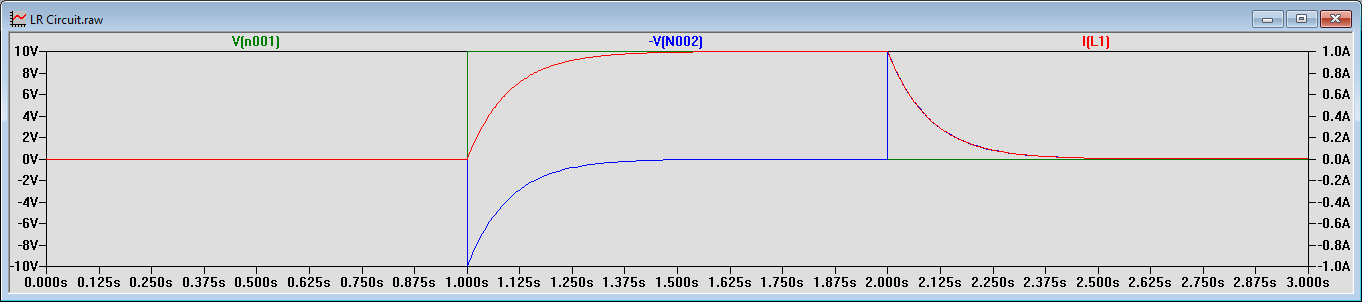
\includegraphics[width=\textwidth]{Images/Circuit.png}

V(001) represents the voltage difference output of the
voltage source. V(002) represents (but is not equivalent to)
the back emf produced by the \SI{1}{H} inductor. I(L1) represents
the current going through the inductor (and therefore
the current going through the whole series
circuit).

LTSpice lets the user measure
current accurately at different points in time. However, it
can be difficult to select an exact point in time (for example,
exactly \SI{1.1}{s}), so any measured values have an uncertainty
of \(\pm \SI{0.010}{s}\). The following updated table displays
measured values along with the theoretical values of the
previous table. (\(t_t\) stands for ``theoretical
time'', \(t_m\) stands for ``measured time'', 
\(i_R(t)\) is Equation 1 and stands for the instantaneous
rising current, \(i_F(t)\) is Equation 2 and stands for
the instantaneous falling current,
\(I\) represents the actual measured current with an
uncertainty of \(\pm \SI{5e-5}{A}\),
and \(\text{RE} =\operatorname{abs}(i - I)/i \)
represents relative error. All \(t_m\) values are
adjusted for rise and fall times of voltage.)

\begin{tabular}{c | c || c | c || c}
    \multicolumn{5}{r}{Rise}\\
    \(t_t\) & \(t_m\) &  \( i_R(-t_t / \tau) \) & \(I\) & RE \\ \hline
    \( \tau = \SI{0.1}{s}\) & \SI{0.10427}{s} & \SI{0.632}{A} & \SI{0.648200}{A} & \num{2.544}\% \\ \hline
    \(2\tau = \SI{0.2}{s}\) & \SI{0.20616}{s} & \SI{0.865}{A} & \SI{0.872719}{A} & \num{0.9315}\% \\ \hline
    \(3\tau = \SI{0.3}{s}\) & \SI{0.30095}{s} & \SI{0.950}{A} & \SI{0.950670}{A} & \num{0.04810}\% \\ \hline
    \(4\tau = \SI{0.4}{s}\) & \SI{0.40047}{s} & \SI{0.982}{A} & \SI{0.981786}{A} & \num{0.01035}\% \\ \hline
    \(5\tau = \SI{0.5}{s}\) & \SI{0.50237}{s} & \SI{0.993}{A} & \SI{0.993410}{A} & \num{0.01490}\% \\ \hline
    \multicolumn{5}{r}{Fall}\\
    \(t_t\) & \(t_m\) &  \( i_F(-t_t / \tau) \) & \(I\) & RE \\ \hline
    \( \tau = \SI{0.1}{s}\) & \SI{0.09479}{s} & \SI{0.368}{A} & \SI{0.387582}{A} & \num{5.356}\% \\ \hline
    \(2\tau = \SI{0.2}{s}\) & \SI{0.20142}{s} & \SI{0.135}{A} & \SI{0.133644}{A} & \num{1.250}\% \\ \hline
    \(3\tau = \SI{0.3}{s}\) & \SI{0.30095}{s} & \SI{0.050}{A} & \SI{0.049213}{A} & \num{1.153}\% \\ \hline
    \(4\tau = \SI{0.4}{s}\) & \SI{0.40284}{s} & \SI{0.018}{A} &\SI{0.0178175}{A} & \num{2.720}\% \\ \hline
    \(5\tau = \SI{0.5}{s}\) & \SI{0.50237}{s} & \SI{0.007}{A} &\SI{0.00656688}{A}& \num{2.539}\% \\
\end{tabular}

The values for relative error are decreasing for rise times
but stay at about \num{2.5}\%; this is likely because the
values for decreasing current are small.

\end{document}
